% TEX compiler = latexmk
% copyright arturo salinas-aguayo 2024
\documentclass[12pt]{article}

\usepackage{graphicx}
\usepackage{amsmath}
\usepackage{array}
\usepackage{amsfonts}
\usepackage{fancyhdr}
\usepackage{geometry}
\usepackage{circuitikz}
\usepackage{subfigure}
\usepackage{caption}
\usepackage{karnaugh-map}
\usepackage{bm}
\usepackage{float}

\geometry{letterpaper, margin=1in}
\graphicspath{ {../images/} }

% Header and Footer
\pagestyle{fancy}
\fancyhf{}
\fancyhead[L]{CSE 2301 - Lab 06: Arithmetic Logic Unit}
\fancyhead[R]{\thepage}
\setlength{\headheight}{15pt}

\author{Arturo Salinas-Aguayo}
\title{Lab 06: Arithmetic Logic Unit}
% theorem set
\newtheorem{example}{Example}
% Example block environment
\newenvironment{examp}
{\vspace{0.5cm}
 \hrule
\vspace{0.5cm}
\begin{example}}
{\hrule
\vspace{0.5cm}
\end{example}}

\begin{document}
\newcommand{\closure}[2][3]{%
	{}\mkern#1mu\overline{\mkern-#1mu#2}}
\newcommand\ncoverline[1]{\mkern1mu\overline{\mkern-1mu#1\mkern-1mu}\mkern1mu}
% Title Page
\begin{titlepage}
	\centering
	\vspace*{3cm}
	\huge\textbf{Lab 06: Arithmetic Logic Unit}\\
	\vspace{5cm}
	\Large\textbf{Arturo Salinas-Aguayo}\\
	\normalsize
	CSE 2301: Principles and Practice of Digital Logic Design\\
	Dr. Mohammad Khan, Section 003L-1248\\
	Electrical and Computer Engineering Department
	\vfill
	
\includegraphics[scale=0.1]{uconnlogo}\\
	College of Engineering, University of Connecticut\\
	\scriptsize{Coded in \LaTeX}
	\vspace*{1cm}
\end{titlepage}
\section*{Theory}
\subsection*{Multiplication Circuits and Output Size Calculation}
A binary multiplier is a combinational circuit that multiplies two binary numbers to produce a product. The circuit performs binary multiplication by breaking down the multiplication process into a series of addition operations, similar to how multiplication is done manually with partial products in decimal.

To create a binary multiplier for any input size:
\begin{itemize}
	\item \textbf{Partial Product Generation:} Each bit of the multiplier (second operand) is ANDed with each bit of the multiplicand (first operand). For an \( m \)-bit multiplicand and an \( n \)-bit multiplier, this creates \( m \times n \) partial products.
	\item \textbf{Summing Partial Products:} These partial products are then aligned according to their bit significance (like shifting in decimal multiplication) and summed to produce the final result. The addition process can be achieved using a series of adders, such as half-adders and full-adders, to accumulate each partial product.
\end{itemize}
\textbf{Output Size Calculation:}
The maximum size of the output in bits is crucial for ensuring that the circuit can handle any possible product without overflow. When multiplying two binary numbers:
\begin{itemize}
	\item Given a  \( m \)-bit multiplicand and an \( n \)-bit multiplier, the resulting product will have a maximum of \( m + n \) bits. This is because multiplying two numbers potentially doubles the value size, which requires more bits to represent accurately.
	\item For example:
	      \begin{itemize}
		      \item A 2x2 binary multiplier (multiplying two 2-bit numbers) will produce a 4-bit product, as \( 2 + 2 = 4 \)
		      \item A 3x4 binary multiplier (multiplying a 3-bit number by a 4-bit number) will produce a 7-bit product, as \( 3 + 4 = 7 \)
	      \end{itemize}
\end{itemize}

Thus, to determine the output size of any binary multiplication circuit, you add the bit lengths of the two operands, ensuring enough bits to represent the highest possible result.

\subsection*{Use of 74153 Chips with Shared Selectors}

The 74153 chip is a dual 4-to-1 multiplexer (MUX) IC, meaning it contains two independent 4:1 MUX circuits within a single chip. However, these multiplexers share the same set of selector inputs, meaning they operate in tandem, controlled by the same selector bits.\\
\textbf{Benefit of Shared Selector Bits:}

In our case, having shared selectors is beneficial because:
By having all the selector lines tied together, we can designate the entire circuit to perform a single function. That is, we can have a universal opcode implementation that will span all three of the muliplexors. In my circuit, I used the shared selector lines to choose between AND, OR, ADD, and MULT operations.\\
\textbf{Modifications for Independent Selectors:}\\
\textbf{Add Separate Selector Lines:} Provide separate control inputs for each MUX, which would require additional control logic. This could inpvolve adding extra multiplexers or decoders to ensure that each MUX has its own dedicated selector input. IE more switches and chips.

In summary, shared selectors on the 74153 chip reduce circuit complexity and are advantageous in applications where synchronized selection is desired, making it a suitable choice for many standard combinational circuits.
\subsection*{Discussion}
\subsubsection*{A 4x4 Bit Combinational Multiplier?}
In my realized 4x4 bit multiplier circuit, two 4-bit binary numbers, \( A = \{A3, A2, A1, A0\} \) and \( B = \{B3, B2, B1, B0\} \), are multiplied using a combination of AND gates for generating partial products and 4-bit full adders for summing these products.

The maximum number this circuit can calculate is \( 15 \times 15 = 225 \), which fits within 8 bits. This is because the bit size of the product equals the sum of the bit sizes of the multiplicand and multiplier.

Each bit of \( A \) is ANDed with each bit of \( B \) to generate 16 partial products.

These partial products are fed into the \textbf{PPBus}, which is then connected to three 4-bit full adders to sum the partial products and produce the final 8-bit product
\[
	P = \{P7, P6, P5, P4, P3, P2, P1, P0\}
\]

The PPBus is organized as follows:
\[
	\text{pp[0..15]} =  pp0, pp1, pp2, \dots, pp15
\]
where each \( pp_{ij} = A_i \cdot B_j \).

The PPBus is a nickname for a data bus representing 15 bits of partial products. The partial products are generated by ANDing each bit of the multiplicand with each bit of the multiplier. The PPBus is then connected to the 4-bit full adders to sum the partial products and produce the final product.
The final product \( P \) is given by:
\[
	P = \{ P7, P6, P5, P4, P3, P2, P1, P0 \}
\]
The LSB of the first partial product flows directly to \( P0 \). The LSB of each adder's sum output contributes to a bit of the final product, while the higher bits are cascaded into the next adder’s inputs until all partial products are summed. The key to this major simplification is actually within the first full adder, by setting A3 to \(0\) a beautiful, cascading circuit can be made.
\subsubsection*{ALU Circuit Design Using 74153 and 74157 Multiplexers}
\begin{center}
	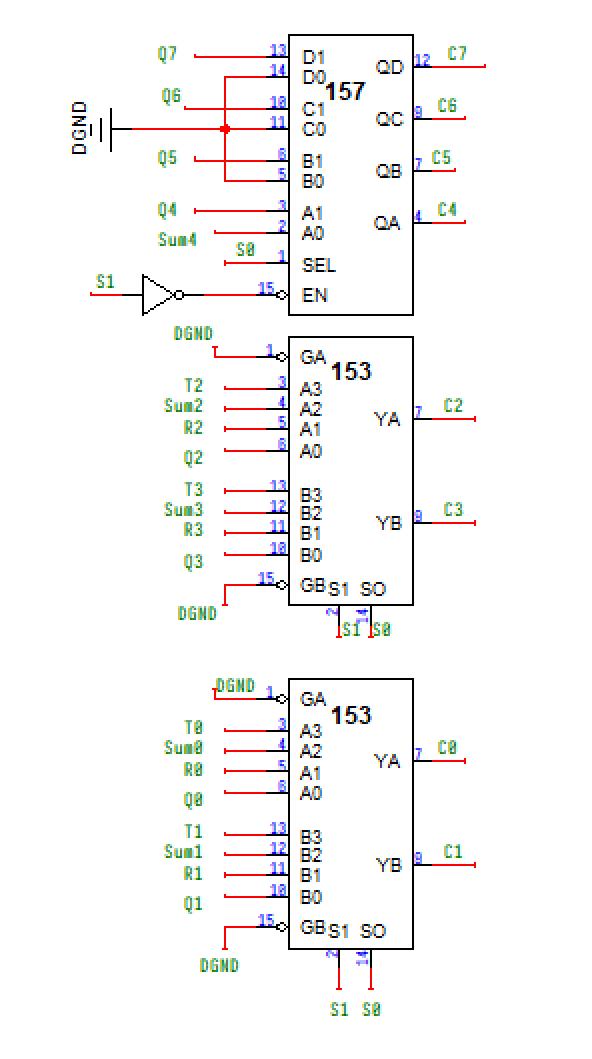
\includegraphics[scale=1]{examp061.png}
\end{center}
The abstraction behind this implementation is such that the S0 bit selects
whether the multiplexer performs a Addition or a Multiplication operation for
the top 4 bits of the ALU. The S1 bit is INV to indicate that whenever the
S1 bit is high, the multiplexer is Enabled. The S1 bit is only high when the
operation should be an ADD or a MULT, so this works.

The 5th Sum bit, Sum4 in the diagram, is fed into the first bit to indicate the
5th bit output, the rest are grounded as the addding 4 bits by 4 bits at most
can give a value of 30, which can be represented with 5 bits.

The rest of the 74153 chips function the same way as the lab apart from the 4th
bit of the Addition operation.

\begin{examp}
	\textbf{8-1 MUX Circuit}

	To implement this function using an 8:1 multiplexer:

	\begin{itemize}
		\item \textbf{Identify Minterms:} The minterms for the function \( F = \sum m(0, 1, 6, 7) \) represent binary combinations of \( CBA \):
		      \begin{itemize}
			      \item \( m(0) = 000 \)
			      \item \( m(1) = 001 \)
			      \item \( m(6) = 110 \)
			      \item \( m(7) = 111 \)
		      \end{itemize}
		      \begin{center}
			      \begin{tabular}{|c|c|c|c|}
				      \hline
				      \( C \) & \( B \) & \( A \) & \( F \) \\
				      \hline
				      0       & 0       & 0       & 1       \\
				      0       & 0       & 1       & 1       \\
				      0       & 1       & 0       & 0       \\
				      0       & 1       & 1       & 0       \\
				      1       & 0       & 0       & 0       \\
				      1       & 0       & 1       & 0       \\
				      1       & 1       & 0       & 1       \\
				      1       & 1       & 1       & 1       \\
				      \hline
			      \end{tabular}
		      \end{center}
		\item \textbf{Multiplexer Inputs:} An 8:1 MUX uses three select inputs (here \( C, B, A \)) to choose from eight data inputs (\( D_0 \) through \( D_7 \)).
		      \begin{itemize}
			      \item \( D_0 = 1 \) (since \( m(0) = 000 \))
			      \item \( D_1 = 1 \) (since \( m(1) = 001 \))
			      \item \( D_6 = 1 \) (since \( m(6) = 110 \))
			      \item \( D_7 = 1 \) (since \( m(7) = 111 \))
			      \item All other inputs (\( D_2, D_3, D_4, D_5 \)) are set to 0.
		      \end{itemize}
		\item \textbf{Conceptual Answer:} Ultimately, our three input bits are connected to the selector
		      bits of the 8-1 MUX. The inputs, \(D_0..D_7\) are connected to logic high
		      or low depending on if the MUX is active high output or output low,
		      but the logic is the same.

	\end{itemize}
\end{examp}

\begin{examp}
	\textbf{4-1 MUX with XOR}

	\begin{enumerate}
		\item \textbf{Determine the MUX Selection:} With \( S_1 = 1 \) and \( S_0 = 0 \), the select lines choose input \( A_2 \).

		\item \textbf{Evaluate Input \( A_2 \):} The input \( A_2 \) is connected to an XOR gate, which outputs \( \closure{X} \oplus Y \). Substitute \( X = 0 \) and \( Y = 1 \):
		      \begin{align*}
			      \closure{X}          & = 1 \quad \text{(since \( X = 0 \))} \\
			      \closure{X} \oplus Y & = 1 \oplus 1 = 0
		      \end{align*}

		\item \textbf{Output \( F \):} Since \( A_2 = 0 \) (from the XOR gate), the output \( F = 0 \) for this selection of inputs.
	\end{enumerate}
\end{examp}

\begin{examp}
	\textbf{Binary Multiplication}
	\begin{itemize}
		\item \(1011_2 (11) \times 1001_2 (9)\)

		      Start by performing line-by-line multiplication as in decimal, then proceed with binary addition:

		      \[
			      \begin{array}{ccccccccc}
				        &                 &   &   &        & 1 & 0 & 1 & 1 \\
				        &                 &   &   & \times & 1 & 0 & 0 & 1 \\
				      \hline
				        & 1 \times 1011_2 &   &   &        & 1 & 0 & 1 & 1 \\
				        & 0 \times 1011_2 &   &   & 0      & 0 & 0 & 0 &   \\
				        & 0 \times 1011_2 &   & 0 & 0      & 0 & 0 &   &   \\
				      + & 1 \times 1011_2 & 1 & 0 & 1      & 1 &   &   &   \\
				      \hline
				        &                 & 1 & 1 & 0      & 1 & 1 & 1 & 1 \\
			      \end{array}
		      \]
		      \[
			      1011_2 \times 1001_2 = 1101111_2
		      \]
		      Therefore, our answer in decimal is 99, but our final result must be in 8 bits, so we append a leading MSB.
		      \[
			      01101111_2
		      \]

	\end{itemize}
\end{examp}
\begin{examp}
	\begin{itemize}
		\item In decimal, \(-15 \times 7 = -105\).
		      Because -15 is negative, we must first take the two's compliment in order to perform the multiplication.
		\item 15 is \(1111_2\), so the two's complement is \(0001_2\) added to the flipped bits of 15 expanded to 8 bits.
		      \[
			      \begin{aligned}
				      00001111_2   & \quad \text{(original number)}         \\
				      \hline
				      11110000_2   & \quad \text{(flipped bits)}            \\
				      + 00000001_2 & \quad \text{(add 1)}                   \\
				      \hline
				      11110001_2   & \quad \text{(two's complement result)} \\
			      \end{aligned}
		      \]
		      The two's complement of \(00001111_2\) is:
		      \[
			      11110001_2
		      \]
		\item Multiply \(11110001_2\) by \(00000111_2\) following binary multiplication rules:
		      \[
			      \begin{array}{c c c c c c c c c c c c c c c c c }
				       &          &  &  &  &  &   &   &   & 1 & 1 & 1 & 1 & 0 & 0 & 0 & 1 \\
				       & \times   &  &  &  &  &   &   &   & 0 & 0 & 0 & 0 & 0 & 1 & 1 & 1 \\
				      \hline

				       & 1 \times &  &  &  &  &   &   &   & 1 & 1 & 1 & 1 & 0 & 0 & 0 & 1 \\

				       & 1 \times &  &  &  &  &   &   & 1 & 1 & 1 & 1 & 0 & 0 & 0 & 1 &   \\
				       & 1 \times &  &  &  &  &   & 1 & 1 & 1 & 1 & 0 & 0 & 0 & 1 &   &   \\
				       & 0 \times &  &  &  &  & 0 & 0 & 0 & 0 & 0 & 0 & 0 & 0 &   &   &   \\
				      \hline
				       &          &  &  &  &  &   &   &   & 1 & 0 & 0 & 1 & 0 & 1 & 1 & 1 \\
			      \end{array}
		      \]
		      There really is no need to keep extending the partial products to the left, as the result is already well over our 8-bits.

		      \(1111_2 \times 0111_2 = 10010111_2\), which, corresponds to
		      \[
			      -105_{10}
		      \]
	\end{itemize}
\end{examp}

\end{document}
% vim: set textwidth=80 wrap formatoptions+=m:
